\documentclass{SKP-beamer}

% --------------------------------------------------- %
%                  Presentation info	              %
% --------------------------------------------------- %
\title[General Disease Prediction System]{Seminar I\\Predicting the Unpredictable \\
	A General Disease Prediction System}
\author{Hitesh Mishra \& Riya Choudhary}
\institute[SIT]{
  Silicon Institute of Technology , Sambalpur
}
\date{\today}
\logo{

\includegraphics[scale=0.5]{SIT_logo.png}
}
\subject{Presentation subject} % metadata

% --------------------------------------------------- %
%                    Title + Schedule                 %
% --------------------------------------------------- %

\begin{document}

\begin{frame}
  \titlepage
\end{frame}


\begin{frame}{Table of Contents}
	\begin{itemize}
		\item Introduction
		\item How it Works
		\item Types
		\item Diabetes Prediction System
		\item Heart Disease Prediction System
		\item Benefits
		\item Challenges
		\item Future Developments
		\item Conclusion
	\end{itemize}
\end{frame}

\begin{frame}{Abstract}
	\begin{itemize}
		Now-a-days, people face various diseases due
		to the environmental condition and their living habits. So
		the prediction of disease at earlier stage becomes
		important task. But the accurate prediction on the basis of
		symptoms becomes too difficult for doctor. 
		The correct
		prediction of disease is the most challenging task. To
		overcome this problem data mining plays an important
		role to predict the disease.
		Due to increase amount
		of data growth in medical and healthcare field the accurate
		analysis on medical data which has been benefits from
		early patient care. With the help of disease data, data
		mining finds hidden pattern information in the huge
		amount of medical data. 
		We proposed general disease
		prediction based on symptoms of the patient. For the
		disease prediction, we use K-Nearest Neighbor (KNN) and
		Convolutional neural network (CNN) machine learning
		algorithm for accurate prediction of disease.
	\end{itemize}
\end{frame}

\begin{frame}{Motivation}
	\begin{itemize}
		\item Most hospitals today employ some sort of hospital information systems to manage their healthcare or patient data. 
		\item These systems typically generate huge amounts of data which take the form of numbers,text, charts and images. 
		\item Unfortunately, these data are rarely used to support clinical decision making. There is a wealth of hidden information in these data that is largely untapped. This raises an important question:
	   “How can we turn data into useful information that can
	   enable healthcare practitioners to make intelligent
	   clinical decisions?” This is the main motivation for this
	research
\end{itemize}
\end{frame}

\begin{frame}{Introduction}
\begin{itemize}
  \item The General Disease Prediction System is an innovative technology that uses advanced artificial intelligence algorithms to predict the occurrence of diseases in individuals.
  
  \item This system is designed to analyze various factors such as age, medical history, lifestyle habits, and environmental conditions to provide accurate predictions
\end{itemize}
\end{frame}



% --------------------------------------------------- %
%                      Presentation                   %
% --------------------------------------------------- %



\begin{frame}{How it Works}
	\begin{itemize}
		\item The General Disease Prediction System works by collecting and analyzing large amounts of data from various sources such as medical records, genetic testing, and environmental sensors.
		\item The system then uses machine learning algorithms to identify patterns and correlations between different variables to accurately predict the likelihood of developing certain diseases.
	\end{itemize}
\end{frame}

\section{Prediction System}

\begin{frame}{General Disease Prediction System}
	\begin{itemize}
	\item Artificial Intelligence made computer more intelligent and can
	enable the computer to think. 
	\item AI study consider machine learning as subfield in numerous research work. Different
	analysts feel that without learning, insight can't be created.
	\item There are numerous kinds of Machine Learning Techniques
	like Unsupervised, Semi Supervised, Supervised,Reinforcement, Evolutionary Learning and Deep Learning.
	\item These learnings are used to classify huge data very fastly. So
	we use K-Nearest Neighbor (KNN) and Convolutional neural
	network (CNN) machine learning algorithm for fast
	classification of big data and accurate prediction of disease.
	\item Because medical data is increasing day by day so usage of that
	for predicting correct disease is crucial task but processing big
	data is very crucial in general so data mining plays very
	important role and classification of large dataset using
	machine learning becomes so easy.
\end{itemize}
\end{frame}

\begin{frame}{System Architecture}
	\begin{center}
	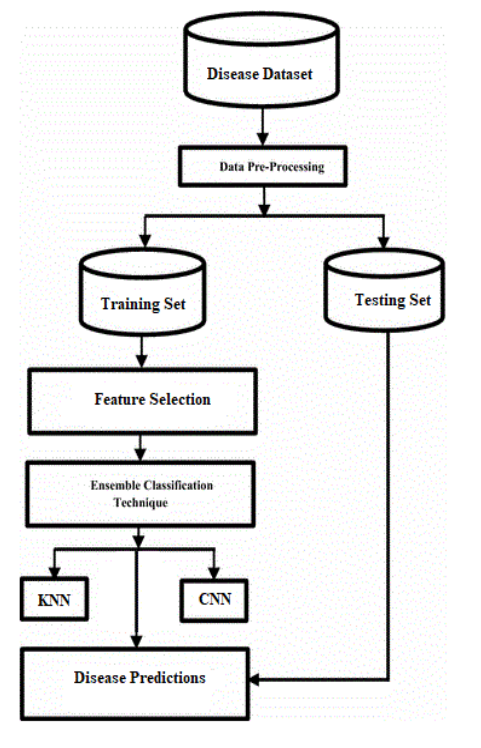
\includegraphics[scale=0.48]{1.png}
\end{center}
\end{frame}

\section{\textbf{Types}}

\begin{frame}{Types of Prediction System}
	\begin{itemize}
		\item Diabetes Prediction System
		\item Heart Disease Prediction System			
	\end{itemize}
\end{frame}



\begin{frame}{Diabetes Prediction System}
	\begin{itemize}
		\item Diabetes is one of deadliest diseases in the
		world. It is not only a disease but also a creator of
		different kinds of diseases like heart attack,
		blindness, kidney diseases, etc.Diabetes Mellitus is defined as a group of metabolic
		disorders mainly caused by abnormal insulin
		secretion and/or action. 
		\item Insulin deficiency results in
		elevated blood glucose levels (hyperglycemia) and
		impaired metabolism of carbohydrates, fat and
		proteins.
		\item There are two major clinical types : \\ 
		--Type 1 diabetes (T1D) \\
		--Type 2 diabetes (T2D) 
		\item According to the etiopathology
		of the disorder. T2D appears to be the most common
		form of diabetes,mainly characterized by insulin resistance. 
		\item The main causes of T2D include lifestyle, physical activity,dietary habits and heredity, whereas T1D is thought to be due to autoimmunological destruction of the Langerhans islets hosting pancreatic beta cells.	
	\end{itemize}
\end{frame}

\begin{frame}{Working Principle}
	\begin{itemize}
		\item Machine learning is the scientific field
		dealing with the ways in which machines learn from
		experience.The purpose of
		machine learning is the construction of computer
		systems that can adapt and learn from their experiences.
		\item We have developed a system using data
		mining which has the ability to predict whether the
		patient has diabetes or not.
		\item Furthermore, predicting
		the disease early leads to treating the patients before
		it becomes critical. Data mining has the ability to
		extract hidden knowledge from a huge amount of
		diabetes-related data.
		\item The aim of this research is to develop a system
		which can predict the diabetic risk level of a patient
		with a higher accuracy. 
		\item This research has focused on
		developing a system based on three classification
		methods namely, Support Vector Machine, Logistic
		regression and Artificial Neural Network algorithms. 
	\end{itemize}
\end{frame}






\begin{frame}{Heart Disease Prediction System}
	\begin{itemize}
		\item Heart disease, alternatively known as cardiovascular disease, encases various conditions that impact the heart and is the primary basis of death worldwide over the span of the past few decades.
		\item  It associates many risk factors in heart disease and a need of the time to get accurate, reliable, and sensible approaches to make an early diagnosis to achieve prompt management of the disease. 
		\item Data mining is a commonly used technique for processing enormous data in the healthcare domain.
		\item Researchers apply several data mining and machine learning techniques to analyse huge complex medical data, helping healthcare professionals to predict heart disease. 
		\item This project will be presenting various attributes related to heart disease, and the model on basis of supervised learning algorithms as Naïve Bayes, decision tree, K-nearest neighbor, and random forest algorithm.
	\end{itemize}
\end{frame}

\begin{frame}{Working Principle}
	\begin{itemize}
		\item For predicting heart attack, significantly 15 attributes are listed
		and with basic data mining technique other approaches e.g. ANN,Time Series, Clustering and Association Rules, soft computing approaches etc. can also be incorporated. 
		\item The outcome of predictive data mining technique on the same dataset reveals that
		Decision Tree outperforms and some time Bayesian classification is having similar accuracy as of decision tree but other predictive methods like KNN, Neural Networks, Classification based on clustering are not performing well.
		\item Decision Tree and Bayesian Classification further improves after applying genetic algorithm to reduce the actual data size to get the optimal subset of attribute sufficient for heart disease prediction.
	\end{itemize}
\end{frame}



\begin{frame}{K-Neighbors Classifier Pseudo code}
	\begin{center}
		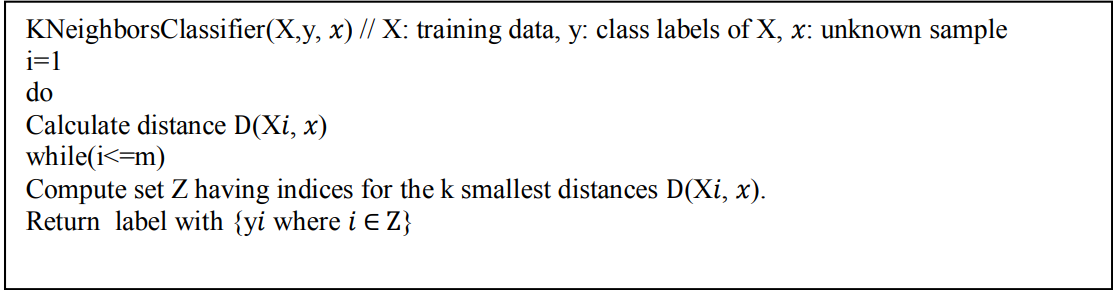
\includegraphics[scale=0.48]{2.png}
	\end{center}
\end{frame}

\section{\textbf{Features}}

\begin{frame}{Features}
	\begin{itemize}
		\item Accurately predicts the spread of diseases. 
		\item It has the ability to analyze large amounts of data in real-time. 
		\item Predict future outbreaks of diseases. 
		\item It has ability to integrate with other healthcare systems, such as electronic health records and hospital information systems. 
		\item This enables it to access a patient's medical history and genetic makeup, which can be used to predict their likelihood of developing certain diseases.
		\item User-friendly interface that makes it easy for healthcare professionals to use. 
		\item The system provides visualizations and dashboards that allow users to quickly and easily interpret complex data. 
		\item It also has built-in analytics tools that enable users to conduct further analysis and refine their predictions over time.
		
	\end{itemize}
\end{frame}

\section{\textbf{Applications}}

\begin{frame}{Applications}
	\begin{itemize}
		\item The general disease prediction system has a wide range of applications in the healthcare industry. One of the primary applications is in disease surveillance, where it can be used to monitor and track the spread of infectious diseases. 
		\item The system can also be used to predict outbreaks of diseases based on historical data and current trends.
		\item Another application of the system is in personalized medicine. By analyzing a patient's genetic makeup and medical history, the system can predict their likelihood of developing certain diseases and recommend personalized treatment plans. 
		\item This can lead to better patient outcomes and more effective use of healthcare resources.
	\end{itemize}
\end{frame}


\section{\textbf{Future Developments}}

\begin{frame}{Future Developments}
	\begin{itemize}
	\item As technology continues to advance, the General Disease Prediction System will likely become even more accurate and effective.
	\item New developments in wearable devices, genetic testing, and artificial intelligence will enable the system to provide even more personalized and precise prediction
    \end{itemize}
\end{frame}

\section{\textbf{Literature Review}}

\begin{frame}{Literature Review}
	\centering
	\resizebox{\columnwidth}{55}{%
		\begin{tabular}{|l|l|l|l|l|l|l|}
			\hline
			\rowcolor[HTML]{87CEEB} 
			{\color[HTML]{333333} Ref. No} &
			Author(s) &
			Year&
			Publisher &
			Objective &
			Proposed Model &
			Impact \\ \hline
			1 &
			Dhiraj ,
			Gajanan ,
			Ektaa&
			\begin{tabular}[c]{@{}l@{}}2010\end{tabular}&
			\begin{tabular}[c]{@{}l@{}}IEEE\end{tabular}&
			\begin{tabular}[c]{@{}l@{}}Design a Disease \\ prediction model\\using dataset for\\ disease prediction\end{tabular} &
			\begin{tabular}[c]{@{}l@{}}Disease prediction by machine\\ learning over big data
				from healthcare \\communities\end{tabular} &
			\begin{tabular}[c]{@{}l@{}}The proposed general disease
				prediction\\ based on symptoms of the patient.\\ For the
				disease prediction,\\ we use K-Nearest Neighbor (KNN)\\ and
				Convolutional neural network (CNN)
			\end{tabular} \\ \hline
			2 &
			B.Qian,X. Wang,N. Cao,H. Li &
			\begin{tabular}[c]{@{}l@{}}2012\end{tabular}&
			\begin{tabular}[c]{@{}l@{}}Springer\end{tabular}&
			\begin{tabular}[c]{@{}l@{}}A
				relative similarity\\ based method for interactive\\ patient risk
				prediction\end{tabular} &
			\begin{tabular}[c]{@{}l@{}}Heart Disease Prediction model \end{tabular} &
			\begin{tabular}[c]{@{}l@{}}A prototype heart disease\\ prediction system is
				developed\\ using three data mining\\ classification
				modeling techniques.\end{tabular} \\ \hline
			3 &
			\begin{tabular}[c]{@{}l@{}}IM. Chen,Y. Ma, Y. Li, D. Wu\end{tabular} &
			\begin{tabular}[c]{@{}l@{}}2017\end{tabular}&
			\begin{tabular}[c]{@{}l@{}} IEEE\end{tabular}&
			\begin{tabular}[c]{@{}l@{}}A Prediction \\ model to predict diabetes\\ in female patients \end{tabular} &
			\begin{tabular}[c]{@{}l@{}}Diabetes Prediction Model for female \\ patients\end{tabular} &
			\begin{tabular}[c]{@{}l@{}}A prototype diabetes prediction model\\ is developed which using decision trees\\ and random forest algorithm to predict the\\ missing values. The model has\\ an accuracy score of 74.4\end{tabular} \\ \hline
		\end{tabular}%
	}
\end{frame}

\section{\textbf{Conclusion}}

\begin{frame}{Conclusion}
	\begin{itemize}
	\item The General Disease Prediction System represents a major breakthrough in the field healthcare, offering numerous benefits for patients and healthcare providers alike.
	\item While there are still challenges to be addressed, the potential impact of this technology on disease prevention and treatment is immense
    \end{itemize}
\end{frame}

\section{\textbf{References}}

\begin{frame}{References}
	\begin{itemize}
	\item Weiguo, F., Wallace, L., Rich, S., Zhongju, Z.: 
	“Tapping the Power of Text Mining”, Communication of the 
	ACM. 49(9), 77-82, 2006. 
	\item Wu, R., Peters, W., Morgan, M.W.: “The Next 
	Generation Clinical Decision Support: Linking Evidence to 
	Best Practice”, Journal Healthcare Information Management. 
	16(4), 50-55, 2002
	\item Chapman, P., Clinton, J., Kerber, R. Khabeza, T., 
	Reinartz, T., Shearer, C., Wirth, R.: “CRISP-DM 1.0: Step 
	by step data mining guide”, SPSS, 1-78, 2000.
	\item  Fayyad, U: “Data Mining and Knowledge Discovery in 
	Databases: Implications fro scientific databases”, Proc. of the 
	9th Int. Conf. on Scientific and Statistical Database 
	Management, Olympia, Washington, USA, 2-11, 1997
	\item Weiguo, F., Wallace, L., Rich, S., Zhongju, Z.: 
	“Tapping the Power of Text Mining”, Communication of the 
	ACM. 49(9), 77-82, 2006.
    \end{itemize}	 
\end{frame}



\section{\textbf{Thank You!!}}
\end{document}
